\documentclass{jsarticle}
\usepackage{amssymb}
\usepackage{graphicx}
\usepackage[dvipdfmx]{color}
\usepackage{here}
\usepackage{tabularx}
\usepackage{amsmath}
\usepackage{amsthm}
\usepackage{url}
\usepackage[hang,small,bf]{caption}
\usepackage[subrefformat=parens]{subcaption}
\usepackage{tikz}
\usepackage{siunitx}
\usepackage{bm}
\usepackage{ascmac}
\usepackage{tasks}
\usepackage[top=15truemm,bottom=20truemm,left=20truemm,right=20truemm]{geometry}
% \usepackage{fancybx}
\usetikzlibrary{shapes.geometric}
\usetikzlibrary {shapes.misc}
\usetikzlibrary{positioning}
\captionsetup{compatibility=false}


\begin{document}
5/31
\settasks{counter-format=(\arabic*)} %「=」の後ろで箇条書きの記号を変更

\section*{Ex4.1}
二次元自律システムを考える。次の平衡点の種類ごとに、
その平衡点が安定、不安定、漸近安定であるかどうかを分類せよ:
\begin{tasks}(3) %()の中で何カラムかを指定
  \task stable node 
  \task unstable node
  \task stable focus
  \task unstable focus 
  \task center
  \task saddle
\end{tasks}
位相ポートレートを用いて、あなたの答えを正当化すること。

{\color{gray}\hrulefill}

\begin{tasks}(3) %()の中で何カラムかを指定
  \task 漸近安定
  \task 不安定
  \task 漸近安定
  \task 不安定
  \task 安定
  \task 不安定
\end{tasks}

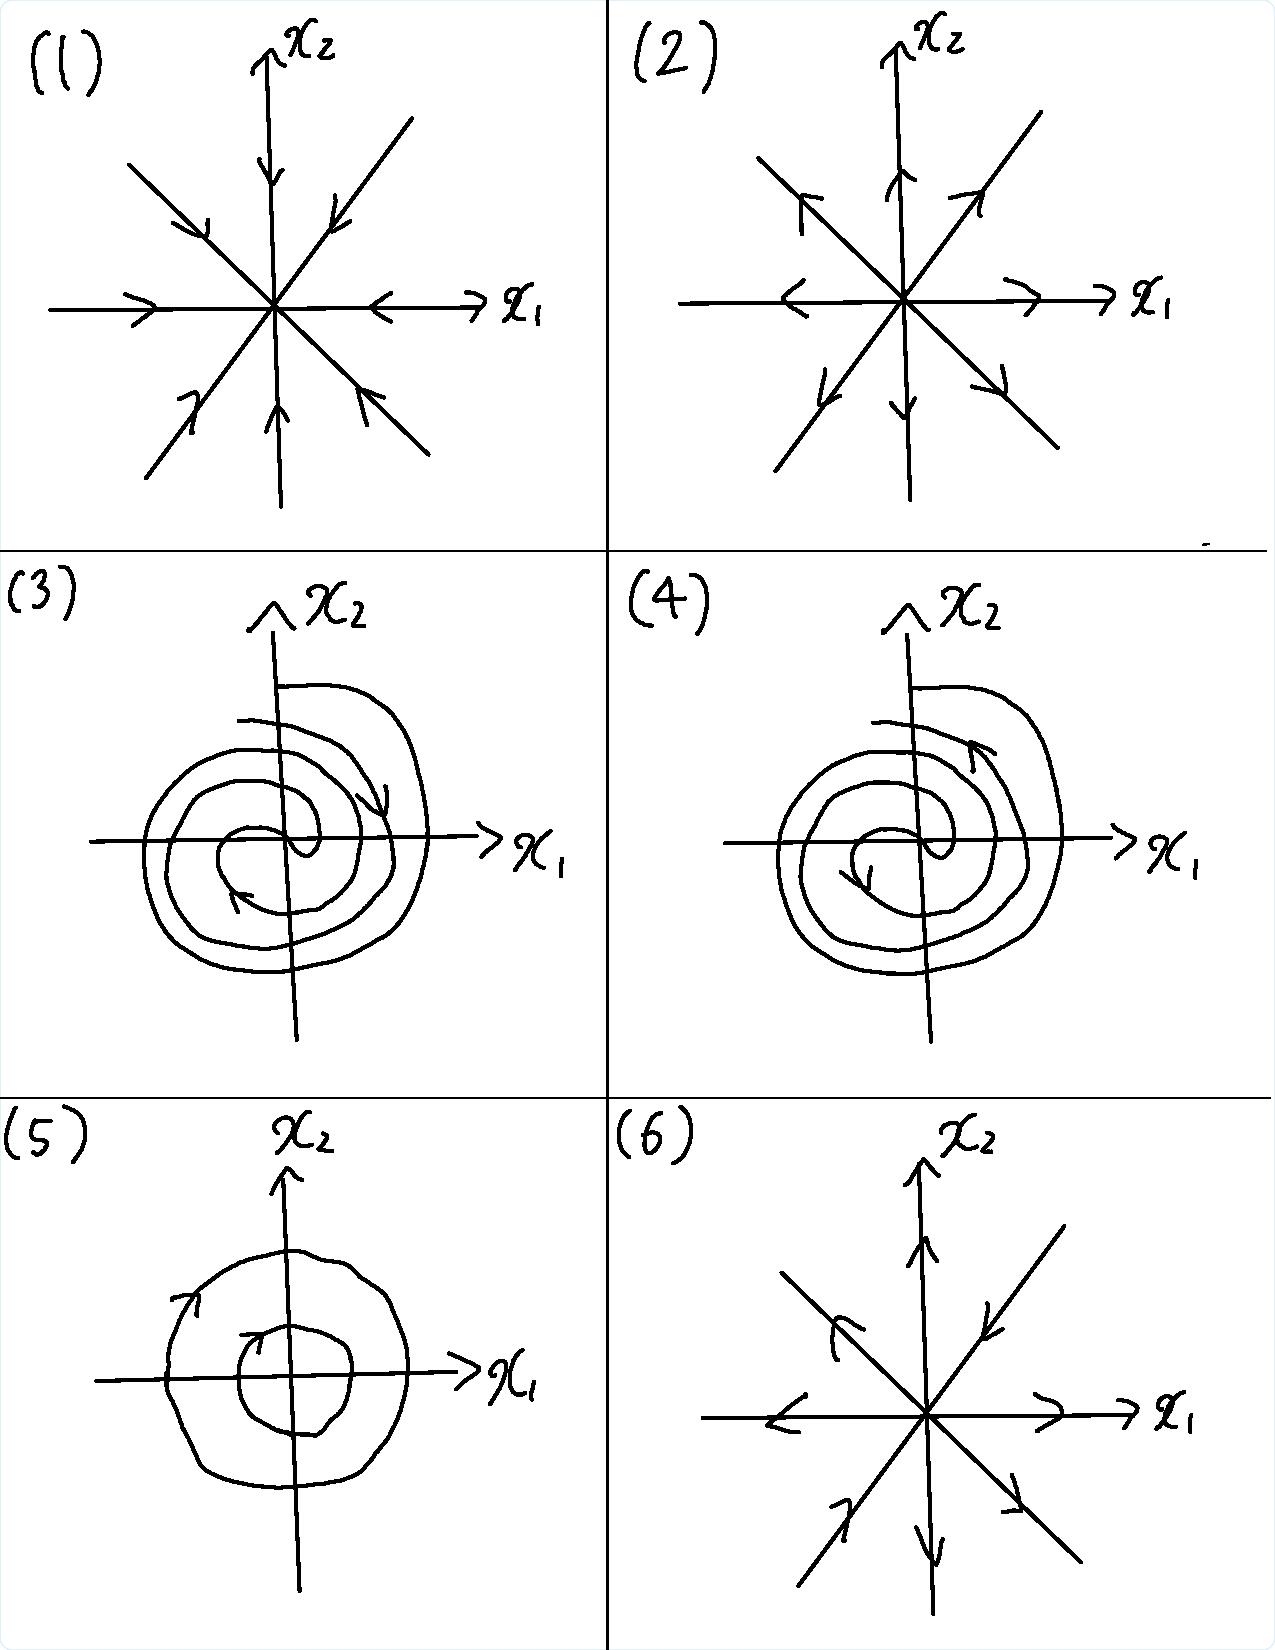
\includegraphics[width=14cm]{fig.pdf}

\newpage
\section*{Ex4.26}

$\dot x = f ( x )$ とし、ここで $f \colon \mathbb R^n \rightarrow \mathbb R^n$
とする。変数変換$z = T(x)$を考える。
ここで、$T ( 0 ) = 0$ であり、$T \colon \mathbb R^n → \mathbb R^n$ 
は原点近傍の微分同相写像である;
すなわち、逆写像 $T^{ - 1} ( \cdot)$ が存在し、
$T ( \cdot )$ と $T ^{- 1} ( \cdot )$ 
は共に連続微分可能である。
変換したシステムは以下である。
\begin{equation*}
  \dot z = \hat f(z) \;,\; \text{where} \hat f(z) = \left.\frac{\partial T}{\partial x}f(x)\right|_{x = T^{-1}(z)}
\end{equation*}

\begin{itemize}
  \item[(a)] $x = 0$ が $\dot x = f ( x )$ の孤立平衡点であるとき、
  かつその時に限り、$z = 0$ が $\dot z = \hat f ( z )$ の孤立平衡点であることを示せ。
  \item[(b)] $x = 0$ が安定(漸近安定または不安定)であるとき、
  かつその時に限り、$z = 0$ が安定(漸近安定または不安定)であることを示せ。
\end{itemize}
{\color{gray}\hrulefill}

(a)\\
$x=0$が平衡点であるとき、$f(0)=0$であり、
$\hat f(0)=0$であるため、$z=0$も平衡点であることが分かる。\\
次に$z=0$でも同様に孤立平衡点かを考えていく。\\
$z=0$が孤立平衡点ではなく、原点近傍に$\hat z \neq 0$の平衡点があると仮定する。
このとき、$\hat f(\hat z) = 0$である。
よって、
\begin{equation*}
  \left.\frac{\partial T}{\partial x}f(x)\right|_{x = T^{-1}(\hat z)} = \hat f(\hat z) = 0
\end{equation*}
であるため、$f( T^{-1}(\hat z)) = 0$であることが分かり、$x=0$が孤立平衡点である
ことと矛盾する。\\
そのため、$z=0$は孤立平衡点である。\\
反対も同様の議論が成立するため、$x=0$が孤立平衡点であるとき、
かつその時に限り、$z=0$が孤立平衡点である。

(b)\\
平衡点$x=0$が安定であるとき、与えられた$\epsilon_1>0$について以下を満たす$\delta_1>0$が存在する。
\begin{equation*}
  \|x(0)\|< \delta_1 \Rightarrow \|x(t)\| < \epsilon_1\;,\;\forall t\geq 0
\end{equation*}
さらに、$T(\cdot)$が連続なので、$\|x(t)\|<\epsilon_1 \Rightarrow \|z(t)\| < \epsilon_2 $
を満たす、$\epsilon_2>0$が存在する。
同様に、$T^{-1}(\cdot)$が連続なので、$ \|z(0)\| < \delta_2 \Rightarrow \|x(0)\|<\delta_1$を満たす、$\delta_2$が存在する。
そのため、
\begin{equation*}
  \|z(0)\| < \delta_2 \Rightarrow \|x(0)\|<\delta_1
  \Rightarrow \|x(t)\| < \epsilon_1
  \Rightarrow \|z(t)\| < \epsilon_2 \;,\;\forall t\geq 0
\end{equation*}
が成り立ち、
平衡点$z=0$が安定であることが分かる。\\
反対も同様の議論が成立するため、平衡点$x=0$が安定であるとき、
かつその時に限り、平衡点$z=0$が安定である。

そのため、平衡点$x=0$が不安定であるとき、
かつその時に限り、平衡点$z=0$が不安定であることも同様に分かる。

つぎに、平衡点$x=0$が漸近安定であるとき、以下を満たす。
\begin{equation*}
  \|x(0)\|< \delta_1 \Rightarrow \lim_{t\rightarrow \infty}x(t) = 0
\end{equation*}
$\|x(t)\|<\epsilon_1 \Rightarrow \|z(t)\| < \epsilon_2 $
が成り立ち、$T ( 0 ) = 0$ であるため、
\begin{equation*}
  \lim_{t\rightarrow \infty}\|x(t)\| = 0 \Rightarrow \lim_{t\rightarrow \infty}\|z(t)\| = 0
\end{equation*}
が成り立ち、
平衡点$z=0$が漸近安定であることが分かる。
反対も同様の議論が成立するため、平衡点$x=0$が漸近安定であるとき、
かつその時に限り、平衡点$z=0$が漸近安定である。

\end{document}